% preamble-exam-zh.tex — 共享 preamble
% 用于所有 exam-zh 模板
%
% 样式策略：
%   屏幕 → 语义彩色（蓝=关键想法，红=易错，绿=路线，灰=提示/教师备注）
%   打印 → 自动降级为黑白（通过 print mode 或 monochrome 选项）

\documentclass{exam-zh}

% ---------- 基础配置 ----------
\examsetup{
  page/size = a4paper,
  page/show-head = false,
  page/show-foot = false,
  sealline/show = false,
  font = times,
  math-font = xits,
}

\usepackage{tcolorbox}
\usepackage{needspace}
\usepackage{graphicx}
\usepackage{tikz}
\usetikzlibrary{calc,intersections,angles,quotes,arrows.meta,decorations.markings,patterns.meta,backgrounds}
\usepackage{pgfplots}
\pgfplotsset{compat=1.18}
\tcbuselibrary{skins,breakable}

% ---------- 打印/屏幕颜色切换 ----------
% 用法：\documentclass[monochrome]{exam-zh} 即可切换为纯黑白
% 注意：不要使用 \if@xxx 放在 makeatother 外部；这里改成普通条件名。
\newif\ifeduprintcolor
\eduprintcolortrue

\makeatletter
\@ifclasswith{exam-zh}{monochrome}{\eduprintcolorfalse}{}
\makeatother

% ---------- 语义颜色定义 ----------
% 屏幕：有色彩区分；打印：降级为灰度
\ifeduprintcolor
  % --- 屏幕彩色模式 ---
  \definecolor{edu-blue}{RGB}{47, 82, 122}       % 关键想法
  \definecolor{edu-blue-bg}{RGB}{243, 246, 252}
  \definecolor{edu-red}{RGB}{180, 40, 40}         % 易错提醒
  \definecolor{edu-red-bg}{RGB}{255, 245, 240}
  \definecolor{edu-green}{RGB}{34, 100, 60}       % 路线图
  \definecolor{edu-green-bg}{RGB}{242, 250, 245}
  \definecolor{edu-orange}{RGB}{160, 90, 0}       % 训练目标
  \definecolor{edu-orange-bg}{RGB}{255, 248, 235}
  \definecolor{edu-gray}{RGB}{100, 100, 100}      % 提示/教师备注
  \definecolor{edu-gray-bg}{RGB}{248, 248, 248}
  \definecolor{edu-purple}{RGB}{90, 50, 120}      % 思考题
  \definecolor{edu-purple-bg}{RGB}{248, 244, 252}
\else
  % --- 打印黑白模式 ---
  \definecolor{edu-blue}{gray}{0.15}
  \definecolor{edu-blue-bg}{gray}{0.96}
  \definecolor{edu-red}{gray}{0.25}
  \definecolor{edu-red-bg}{gray}{0.97}
  \definecolor{edu-green}{gray}{0.20}
  \definecolor{edu-green-bg}{gray}{0.97}
  \definecolor{edu-orange}{gray}{0.25}
  \definecolor{edu-orange-bg}{gray}{0.98}
  \definecolor{edu-gray}{gray}{0.40}
  \definecolor{edu-gray-bg}{gray}{0.97}
  \definecolor{edu-purple}{gray}{0.30}
  \definecolor{edu-purple-bg}{gray}{0.98}
\fi
\colorlet{edu-diagram-muted}{edu-gray}

% ---------- TikZ diagram semantic macros ----------
\definecolor{edu-diagram-ink}{RGB}{17,24,39}
\definecolor{edu-diagram-marker}{RGB}{220,38,38}
\definecolor{edu-diagram-angle}{RGB}{5,150,105}
\tikzset{
  diagram point/.style={fill=edu-diagram-ink},
  diagram tick/.style={draw=edu-diagram-marker,line width=0.9pt,line cap=round},
  diagram segment/.style={draw=edu-diagram-ink,line cap=round},
  point label/.style={inner sep=1pt},
  condition label/.style={inner sep=1pt}
}
\providecommand{\DrawSegment}[3][]{\draw[diagram segment,#1] (#2) -- (#3);}
\providecommand{\DrawDashedSegment}[3][]{\draw[diagram segment,dashed,#1] (#2) -- (#3);}
\providecommand{\Triangle}[4][]{\path[#1] (#2) -- (#3) -- (#4) -- cycle;}
\providecommand{\Quadrilateral}[5][]{\path[#1] (#2) -- (#3) -- (#4) -- (#5) -- cycle;}
\providecommand{\PolygonPath}[2][]{\path[#1] #2 -- cycle;}
\providecommand{\DiagramPointRadius}{0.052cm}
\providecommand{\PointDot}[2][]{\fill[diagram point,#1] (#2) circle[radius=\DiagramPointRadius];}
\providecommand{\PointLabel}[3][]{\node[point label,#1] at (#2) {#3};}
\providecommand{\SegmentLabel}[4][]{\node[condition label,#1] at ($(#2)!0.5!(#3)$) {#4};}
\providecommand{\CoordinateTag}[3][]{\node[condition label,#1] at (#2) {#3};}
\providecommand{\AngleMark}[4][]{\pic[draw=edu-diagram-angle,line width=0.9pt,angle radius=0.48cm,#1] {angle=#2--#3--#4};}
\providecommand{\AngleLabel}[5][]{\pic["{#5}",draw=none,angle radius=0.64cm,#1] {angle=#2--#3--#4};}
\providecommand{\RightAngleMark}[4][]{\pic[draw=edu-diagram-marker,line width=0.9pt,angle radius=0.28cm,#1] {right angle=#2--#3--#4};}
\providecommand{\EqualTick}[3][]{%
  \path[postaction={decorate},decoration={markings,mark=at position .5 with {\draw[diagram tick,#1] (0pt,-4pt) -- (0pt,4pt);}}] (#2) -- (#3);%
}
\providecommand{\DoubleEqualTick}[3][]{%
  \path[postaction={decorate},decoration={markings,mark=at position .46 with {\draw[diagram tick,#1] (0pt,-4pt) -- (0pt,4pt);},mark=at position .54 with {\draw[diagram tick,#1] (0pt,-4pt) -- (0pt,4pt);}}] (#2) -- (#3);%
}
\providecommand{\TripleEqualTick}[3][]{%
  \path[postaction={decorate},decoration={markings,mark=at position .43 with {\draw[diagram tick,#1] (0pt,-4pt) -- (0pt,4pt);},mark=at position .5 with {\draw[diagram tick,#1] (0pt,-4pt) -- (0pt,4pt);},mark=at position .57 with {\draw[diagram tick,#1] (0pt,-4pt) -- (0pt,4pt);}}] (#2) -- (#3);%
}
\providecommand{\ParallelMark}[3][]{\EqualTick[#1]{#2}{#3}}
\providecommand{\NamedSegmentPath}[3]{\path[name path=#1] (#2) -- (#3);}
\providecommand{\IntersectPaths}[3]{\path[name intersections={of=#2 and #3, by=#1}];}

% ---------- 自定义教学环境 ----------
% 共性：enhanced + breakable（跨页不断裂）

% 原题卡片 — 强边框，突出显示
\newtcolorbox{problemcard}{
  enhanced, breakable,
  colback=edu-blue-bg,
  colframe=edu-blue,
  boxrule=1.2pt,
  arc=0pt,
  left=3mm, right=3mm, top=3mm, bottom=3mm,
}

% 解题路线图 — 左边线 + 浅底
\newtcolorbox{routebox}{
  enhanced, breakable,
  colback=edu-green-bg,
  colframe=edu-green!30,
  boxrule=0pt,
  borderline west={2.5pt}{0pt}{edu-green},
  left=3mm, right=3mm, top=3mm, bottom=3mm,
}

% 关键想法 — 蓝色左边线
\newtcolorbox{keyideabox}{
  enhanced, breakable,
  colback=edu-blue-bg,
  colframe=edu-blue!30,
  boxrule=0pt,
  borderline west={2.5pt}{0pt}{edu-blue},
  left=3mm, right=3mm, top=3mm, bottom=3mm,
}

% 易错提醒 — 红色左边线
\newtcolorbox{mistakebox}{
  enhanced, breakable,
  colback=edu-red-bg,
  colframe=edu-red!20,
  boxrule=0pt,
  borderline west={3pt}{0pt}{edu-red},
  left=3mm, right=3mm, top=2.5mm, bottom=2.5mm,
}

% 提示 — 灰色虚线左边线
\newtcolorbox{hintbox}{
  enhanced, breakable,
  colback=edu-gray-bg,
  colframe=edu-gray!20,
  boxrule=0pt,
  borderline west={2pt}{0pt}{edu-gray, dashed},
  left=3mm, right=3mm, top=2mm, bottom=2mm,
}

% 思考题 — 紫色虚线左边线
\newtcolorbox{thinkbox}{
  enhanced, breakable,
  colback=edu-purple-bg,
  colframe=edu-purple!20,
  boxrule=0pt,
  borderline west={2pt}{0pt}{edu-purple, dashed},
  left=2.5mm, right=2.5mm, top=2.5mm, bottom=2.5mm,
}

% 教师备注 — 灰色左边线，小字
\newtcolorbox{teachernote}{
  enhanced, breakable,
  colback=edu-gray-bg,
  colframe=edu-gray!15,
  boxrule=0pt,
  borderline west={2pt}{0pt}{edu-gray!60},
  left=2.5mm, right=2.5mm, top=2.5mm, bottom=2.5mm,
  fontupper=\small,
  colupper=black!60,
}

% 训练目标 — 橙色左边线，小字
\newtcolorbox{traininggoal}{
  enhanced, breakable,
  colback=edu-orange-bg,
  colframe=edu-orange!15,
  boxrule=0pt,
  borderline west={1.5pt}{0pt}{edu-orange},
  left=2mm, right=2mm, top=1mm, bottom=1mm,
  fontupper=\small,
}

% 答题区 — 无边框，纯留白
\newcommand{\answerarea}[1][40mm]{%
  \vspace{2mm}%
  \begin{tcolorbox}[
    enhanced, breakable,
    colback=white,
    colframe=white,
    boxrule=0pt,
    height=#1,
    valign=top,
    bottom=0mm,
    after skip=0mm,
  ]
  \end{tcolorbox}%
}

\newsavebox{\diagramtikzbox}

\newenvironment{diagramcoltikz}[2]{%
  \begin{minipage}[t]{#1}
    \vspace{0pt}\centering
    \def\diagramcaption{#2}%
    \begin{lrbox}{\diagramtikzbox}%
}{%
    \end{lrbox}%
    \usebox{\diagramtikzbox}%
    \ifx\diagramcaption\empty\else
      \par\vspace{1mm}{\scriptsize\color{edu-diagram-muted}\diagramcaption}
    \fi
  \end{minipage}%
}

\newenvironment{diagramrowtikz}[3]{%
  \begin{minipage}[t]{#1}
    \vspace{0pt}\centering
    \def\diagramlabel{#2}%
    \def\diagramcaption{#3}%
    \begin{lrbox}{\diagramtikzbox}%
}{%
    \end{lrbox}%
    \usebox{\diagramtikzbox}%
    \ifx\diagramlabel\empty\else
      \par\vspace{1mm}{\scriptsize\bfseries\diagramlabel}
    \fi
    \ifx\diagramcaption\empty\else
      \par\vspace{0.5mm}{\scriptsize\color{edu-diagram-muted}\diagramcaption}
    \fi
  \end{minipage}%
}

\newenvironment{answerareawithdiagramtikz}[3]{%
  \par\vspace{2mm}%
  \noindent
  \begin{minipage}[t]{\dimexpr\linewidth-#2-6mm\relax}
    \vspace{0pt}\rule{0pt}{#1}
  \end{minipage}\hfill
  \begin{diagramcoltikz}{#2}{#3}
}{%
  \end{diagramcoltikz}
  \par\vspace{2mm}%
}

% ---------- 字体设置 ----------
% exam-zh (ctexbook) already sets CJK fonts via ctex.
% Only override if specific fonts are needed.
% macOS: Songti SC, STHeiti, STFangsong
% Linux: SimSun, SimHei, FangSong

% ---------- 页面设置 ----------
% exam-zh (ctexbook) already loads geometry.
% Override margins if needed:
% \geometry{top=16mm, bottom=16mm, left=14mm, right=14mm}

\examsetup{
  question/show-answer = false,
  fillin/show-answer = false,
  solution/show-solution = hide,
}

% ---------- 教师版解答样式 ----------
\newtcolorbox{solutionblock}{
  enhanced, breakable,
  colback=edu-blue-bg,
  colframe=edu-blue!25,
  boxrule=0pt,
  borderline west={2pt}{0pt}{edu-blue!50},
  arc=0pt,
  left=3mm, right=3mm, top=2mm, bottom=2mm,
  before skip=2mm,
  after skip=3mm,
  fontupper=\small,
}

% 解答步骤编号
\newcounter{solstep}
\newcommand{\solstep}[2]{%
  \stepcounter{solstep}%
  \par\medskip
  \noindent\hangindent=6mm
  {\color{edu-blue}\bfseries\textcircled{\scriptsize\thesolstep}\enspace #1}\enspace #2\par
}

\begin{document}

\section*{线段和角份数化填空练习}

\section*{一、看图标份数并填比例方程}

\needspace{8\baselineskip}

\begin{problem}[points=6]
  \noindent
  \begin{minipage}[t]{\dimexpr\linewidth-60mm-6mm\relax}
    \vspace{0pt}
    点 $A,B,C$ 在同一直线上，$B$ 在 $A,C$ 之间。若 $AB:BC=2:5$，且 $AC=49$，求 $AB$。  图上份数：____；比例方程：________________；答案：____。
  \end{minipage}\hfill
  \begin{diagramcoltikz}{60mm}{在图上标：左段 2 份，右段 5 份。}
  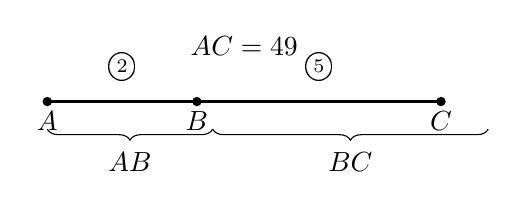
\begin{tikzpicture}[x=1cm,y=1cm,baseline=(current bounding box.center)]
  \draw[line width=1.05pt] (0,0) -- (5.0,0);
  \fill (0,0) circle (1.7pt) node[below] {$A$};
  \fill (1.9,0) circle (1.7pt) node[below] {$B$};
  \fill (5.0,0) circle (1.7pt) node[below] {$C$};
  \draw[decorate,decoration={brace,amplitude=4pt,mirror}] (0,-0.35) -- (2.1,-0.35) node[midway,below=5pt] {$AB$};
  \draw[decorate,decoration={brace,amplitude=4pt,mirror}] (2.1,-0.35) -- (5.6,-0.35) node[midway,below=5pt] {$BC$};
  \node[above=4pt] at (0.95,0) {\textcircled{\scriptsize 2}};
  \node[above=4pt] at (3.45,0) {\textcircled{\scriptsize 5}};
  \node[above=13pt] at (2.5,0) {$AC=49$};
\end{tikzpicture}
  \end{diagramcoltikz}
  \par\medskip
\end{problem}


\needspace{8\baselineskip}

\begin{problem}[points=6]
  \noindent
  \begin{minipage}[t]{\dimexpr\linewidth-60mm-6mm\relax}
    \vspace{0pt}
    点 $A,B,C$ 在同一直线上，$B$ 在 $A,C$ 之间。若 $AB:BC=3:4$，且 $AC=63$，求 $BC$。  图上份数：____；比例方程：________________；答案：____。
  \end{minipage}\hfill
  \begin{diagramcoltikz}{60mm}{在图上标：左段 3 份，右段 4 份。}
  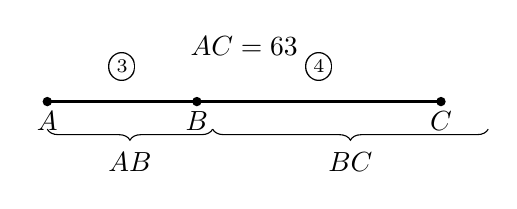
\begin{tikzpicture}[x=1cm,y=1cm,baseline=(current bounding box.center)]
  \draw[line width=1.05pt] (0,0) -- (5.0,0);
  \fill (0,0) circle (1.7pt) node[below] {$A$};
  \fill (1.9,0) circle (1.7pt) node[below] {$B$};
  \fill (5.0,0) circle (1.7pt) node[below] {$C$};
  \draw[decorate,decoration={brace,amplitude=4pt,mirror}] (0,-0.35) -- (2.1,-0.35) node[midway,below=5pt] {$AB$};
  \draw[decorate,decoration={brace,amplitude=4pt,mirror}] (2.1,-0.35) -- (5.6,-0.35) node[midway,below=5pt] {$BC$};
  \node[above=4pt] at (0.95,0) {\textcircled{\scriptsize 3}};
  \node[above=4pt] at (3.45,0) {\textcircled{\scriptsize 4}};
  \node[above=13pt] at (2.5,0) {$AC=63$};
\end{tikzpicture}
  \end{diagramcoltikz}
  \par\medskip
\end{problem}


\needspace{8\baselineskip}

\begin{problem}[points=6]
  \noindent
  \begin{minipage}[t]{\dimexpr\linewidth-60mm-6mm\relax}
    \vspace{0pt}
    点 $A,B,C$ 在同一直线上，$B$ 在 $A,C$ 之间。若 $7AB=2BC$，且 $AC=54$，求 $AB$。  图上份数：____；比例方程：________________；答案：____。
  \end{minipage}\hfill
  \begin{diagramcoltikz}{60mm}{在图上标：左段 2 份，右段 7 份。}
  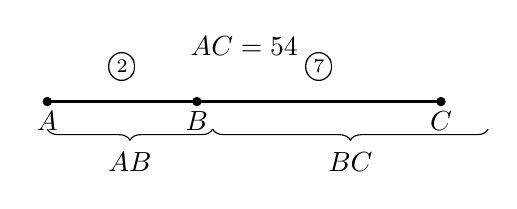
\begin{tikzpicture}[x=1cm,y=1cm,baseline=(current bounding box.center)]
  \draw[line width=1.05pt] (0,0) -- (5.0,0);
  \fill (0,0) circle (1.7pt) node[below] {$A$};
  \fill (1.9,0) circle (1.7pt) node[below] {$B$};
  \fill (5.0,0) circle (1.7pt) node[below] {$C$};
  \draw[decorate,decoration={brace,amplitude=4pt,mirror}] (0,-0.35) -- (2.1,-0.35) node[midway,below=5pt] {$AB$};
  \draw[decorate,decoration={brace,amplitude=4pt,mirror}] (2.1,-0.35) -- (5.6,-0.35) node[midway,below=5pt] {$BC$};
  \node[above=4pt] at (0.95,0) {\textcircled{\scriptsize 2}};
  \node[above=4pt] at (3.45,0) {\textcircled{\scriptsize 7}};
  \node[above=13pt] at (2.5,0) {$AC=54$};
\end{tikzpicture}
  \end{diagramcoltikz}
  \par\medskip
\end{problem}


\needspace{8\baselineskip}

\begin{problem}[points=6]
  \noindent
  \begin{minipage}[t]{\dimexpr\linewidth-60mm-6mm\relax}
    \vspace{0pt}
    点 $A,B,C$ 在同一直线上，$B$ 在 $A,C$ 之间。若 $3AB=5BC$，且 $AC=48$，求 $BC$。  图上份数：____；比例方程：________________；答案：____。
  \end{minipage}\hfill
  \begin{diagramcoltikz}{60mm}{在图上标：左段 5 份，右段 3 份。}
  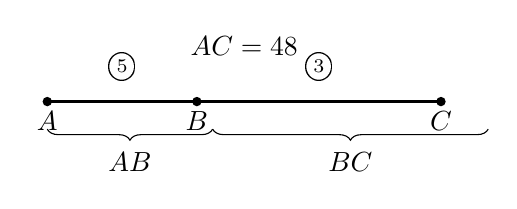
\begin{tikzpicture}[x=1cm,y=1cm,baseline=(current bounding box.center)]
  \draw[line width=1.05pt] (0,0) -- (5.0,0);
  \fill (0,0) circle (1.7pt) node[below] {$A$};
  \fill (1.9,0) circle (1.7pt) node[below] {$B$};
  \fill (5.0,0) circle (1.7pt) node[below] {$C$};
  \draw[decorate,decoration={brace,amplitude=4pt,mirror}] (0,-0.35) -- (2.1,-0.35) node[midway,below=5pt] {$AB$};
  \draw[decorate,decoration={brace,amplitude=4pt,mirror}] (2.1,-0.35) -- (5.6,-0.35) node[midway,below=5pt] {$BC$};
  \node[above=4pt] at (0.95,0) {\textcircled{\scriptsize 5}};
  \node[above=4pt] at (3.45,0) {\textcircled{\scriptsize 3}};
  \node[above=13pt] at (2.5,0) {$AC=48$};
\end{tikzpicture}
  \end{diagramcoltikz}
  \par\medskip
\end{problem}


\needspace{8\baselineskip}

\begin{problem}[points=6]
  \noindent
  \begin{minipage}[t]{\dimexpr\linewidth-60mm-6mm\relax}
    \vspace{0pt}
    射线 $OB$ 在 $\angle AOC$ 内部。若 $4\angle AOB=3\angle BOC$，且 $\angle AOC=91^\circ$，求 $\angle AOB$。  图上份数：____；比例方程：________________；答案：____。
  \end{minipage}\hfill
  \begin{diagramcoltikz}{60mm}{在图上标：左角 3 份，右角 4 份。}
  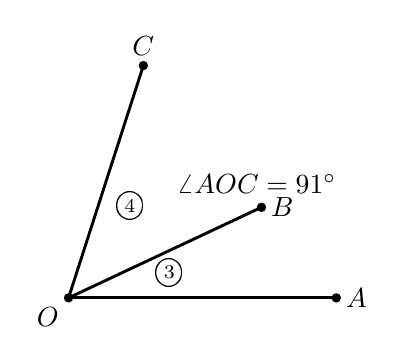
\begin{tikzpicture}[x=1cm,y=1cm,baseline=(current bounding box.center)]
  \coordinate (O) at (0,0);
  \coordinate (A) at (3.4,0);
  \coordinate (B) at (2.45,1.15);
  \coordinate (C) at (0.95,2.95);
  \draw[line width=1.05pt] (O) -- (A);
  \draw[line width=1.05pt] (O) -- (B);
  \draw[line width=1.05pt] (O) -- (C);
  \fill (O) circle (1.7pt) node[below left] {$O$};
  \fill (A) circle (1.7pt) node[right] {$A$};
  \fill (B) circle (1.7pt) node[right] {$B$};
  \fill (C) circle (1.7pt) node[above] {$C$};
  \node at (1.28,0.28) {\textcircled{\scriptsize 3}};
  \node at (0.78,1.12) {\textcircled{\scriptsize 4}};
  \node[right] at (1.25,1.45) {$\angle AOC=91^\circ$};
\end{tikzpicture}
  \end{diagramcoltikz}
  \par\medskip
\end{problem}


\needspace{8\baselineskip}

\begin{problem}[points=6]
  \noindent
  \begin{minipage}[t]{\dimexpr\linewidth-60mm-6mm\relax}
    \vspace{0pt}
    射线 $OB$ 在 $\angle AOC$ 内部。若 $5\angle AOB=2\angle BOC$，且 $\angle AOC=112^\circ$，求 $\angle BOC$。  图上份数：____；比例方程：________________；答案：____。
  \end{minipage}\hfill
  \begin{diagramcoltikz}{60mm}{在图上标：左角 2 份，右角 5 份。}
  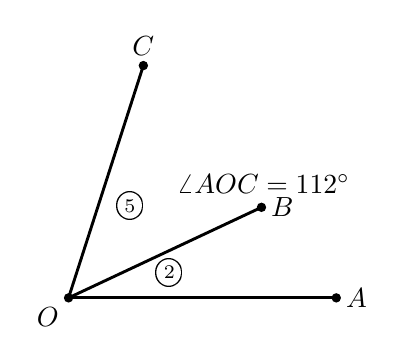
\begin{tikzpicture}[x=1cm,y=1cm,baseline=(current bounding box.center)]
  \coordinate (O) at (0,0);
  \coordinate (A) at (3.4,0);
  \coordinate (B) at (2.45,1.15);
  \coordinate (C) at (0.95,2.95);
  \draw[line width=1.05pt] (O) -- (A);
  \draw[line width=1.05pt] (O) -- (B);
  \draw[line width=1.05pt] (O) -- (C);
  \fill (O) circle (1.7pt) node[below left] {$O$};
  \fill (A) circle (1.7pt) node[right] {$A$};
  \fill (B) circle (1.7pt) node[right] {$B$};
  \fill (C) circle (1.7pt) node[above] {$C$};
  \node at (1.28,0.28) {\textcircled{\scriptsize 2}};
  \node at (0.78,1.12) {\textcircled{\scriptsize 5}};
  \node[right] at (1.25,1.45) {$\angle AOC=112^\circ$};
\end{tikzpicture}
  \end{diagramcoltikz}
  \par\medskip
\end{problem}


\needspace{8\baselineskip}

\begin{problem}[points=6]
  \noindent
  \begin{minipage}[t]{\dimexpr\linewidth-60mm-6mm\relax}
    \vspace{0pt}
    点 $A,B,C$ 在同一直线上，$B$ 在 $A,C$ 之间。若 $AB:BC=4:5$，且 $AC=72$，求 $AB$。  图上份数：____；比例方程：________________；答案：____。
  \end{minipage}\hfill
  \begin{diagramcoltikz}{60mm}{在图上标：左段 4 份，右段 5 份。}
  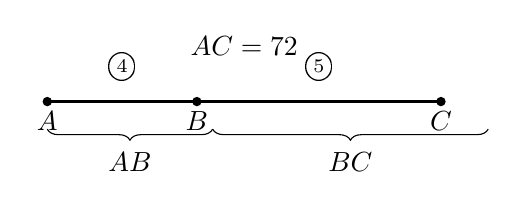
\begin{tikzpicture}[x=1cm,y=1cm,baseline=(current bounding box.center)]
  \draw[line width=1.05pt] (0,0) -- (5.0,0);
  \fill (0,0) circle (1.7pt) node[below] {$A$};
  \fill (1.9,0) circle (1.7pt) node[below] {$B$};
  \fill (5.0,0) circle (1.7pt) node[below] {$C$};
  \draw[decorate,decoration={brace,amplitude=4pt,mirror}] (0,-0.35) -- (2.1,-0.35) node[midway,below=5pt] {$AB$};
  \draw[decorate,decoration={brace,amplitude=4pt,mirror}] (2.1,-0.35) -- (5.6,-0.35) node[midway,below=5pt] {$BC$};
  \node[above=4pt] at (0.95,0) {\textcircled{\scriptsize 4}};
  \node[above=4pt] at (3.45,0) {\textcircled{\scriptsize 5}};
  \node[above=13pt] at (2.5,0) {$AC=72$};
\end{tikzpicture}
  \end{diagramcoltikz}
  \par\medskip
\end{problem}


\needspace{8\baselineskip}

\begin{problem}[points=6]
  \noindent
  \begin{minipage}[t]{\dimexpr\linewidth-60mm-6mm\relax}
    \vspace{0pt}
    点 $A,B,C$ 在同一直线上，$B$ 在 $A,C$ 之间。若 $8AB=3BC$，且 $AC=88$，求 $BC$。  图上份数：____；比例方程：________________；答案：____。
  \end{minipage}\hfill
  \begin{diagramcoltikz}{60mm}{在图上标：左段 3 份，右段 8 份。}
  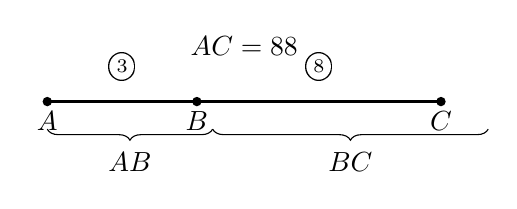
\begin{tikzpicture}[x=1cm,y=1cm,baseline=(current bounding box.center)]
  \draw[line width=1.05pt] (0,0) -- (5.0,0);
  \fill (0,0) circle (1.7pt) node[below] {$A$};
  \fill (1.9,0) circle (1.7pt) node[below] {$B$};
  \fill (5.0,0) circle (1.7pt) node[below] {$C$};
  \draw[decorate,decoration={brace,amplitude=4pt,mirror}] (0,-0.35) -- (2.1,-0.35) node[midway,below=5pt] {$AB$};
  \draw[decorate,decoration={brace,amplitude=4pt,mirror}] (2.1,-0.35) -- (5.6,-0.35) node[midway,below=5pt] {$BC$};
  \node[above=4pt] at (0.95,0) {\textcircled{\scriptsize 3}};
  \node[above=4pt] at (3.45,0) {\textcircled{\scriptsize 8}};
  \node[above=13pt] at (2.5,0) {$AC=88$};
\end{tikzpicture}
  \end{diagramcoltikz}
  \par\medskip
\end{problem}


\needspace{8\baselineskip}

\begin{problem}[points=6]
  \noindent
  \begin{minipage}[t]{\dimexpr\linewidth-60mm-6mm\relax}
    \vspace{0pt}
    射线 $OB$ 在 $\angle AOC$ 内部。若 $\angle AOB:\angle BOC=5:6$，且 $\angle AOC=132^\circ$，求 $\angle AOB$。  图上份数：____；比例方程：________________；答案：____。
  \end{minipage}\hfill
  \begin{diagramcoltikz}{60mm}{在图上标：左角 5 份，右角 6 份。}
  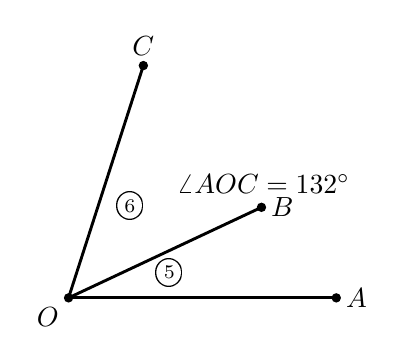
\begin{tikzpicture}[x=1cm,y=1cm,baseline=(current bounding box.center)]
  \coordinate (O) at (0,0);
  \coordinate (A) at (3.4,0);
  \coordinate (B) at (2.45,1.15);
  \coordinate (C) at (0.95,2.95);
  \draw[line width=1.05pt] (O) -- (A);
  \draw[line width=1.05pt] (O) -- (B);
  \draw[line width=1.05pt] (O) -- (C);
  \fill (O) circle (1.7pt) node[below left] {$O$};
  \fill (A) circle (1.7pt) node[right] {$A$};
  \fill (B) circle (1.7pt) node[right] {$B$};
  \fill (C) circle (1.7pt) node[above] {$C$};
  \node at (1.28,0.28) {\textcircled{\scriptsize 5}};
  \node at (0.78,1.12) {\textcircled{\scriptsize 6}};
  \node[right] at (1.25,1.45) {$\angle AOC=132^\circ$};
\end{tikzpicture}
  \end{diagramcoltikz}
  \par\medskip
\end{problem}


\needspace{8\baselineskip}

\begin{problem}[points=6]
  \noindent
  \begin{minipage}[t]{\dimexpr\linewidth-60mm-6mm\relax}
    \vspace{0pt}
    点 $A,B,C$ 在同一直线上，$B$ 在 $A,C$ 之间。若 $6AB=5BC$，且 $AC=99$，求 $AB$。  图上份数：____；比例方程：________________；答案：____。
  \end{minipage}\hfill
  \begin{diagramcoltikz}{60mm}{在图上标：左段 5 份，右段 6 份。}
  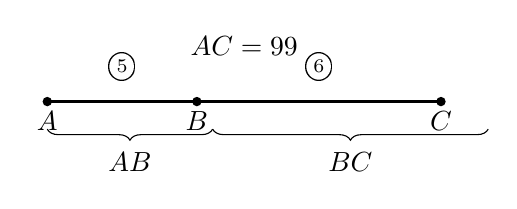
\begin{tikzpicture}[x=1cm,y=1cm,baseline=(current bounding box.center)]
  \draw[line width=1.05pt] (0,0) -- (5.0,0);
  \fill (0,0) circle (1.7pt) node[below] {$A$};
  \fill (1.9,0) circle (1.7pt) node[below] {$B$};
  \fill (5.0,0) circle (1.7pt) node[below] {$C$};
  \draw[decorate,decoration={brace,amplitude=4pt,mirror}] (0,-0.35) -- (2.1,-0.35) node[midway,below=5pt] {$AB$};
  \draw[decorate,decoration={brace,amplitude=4pt,mirror}] (2.1,-0.35) -- (5.6,-0.35) node[midway,below=5pt] {$BC$};
  \node[above=4pt] at (0.95,0) {\textcircled{\scriptsize 5}};
  \node[above=4pt] at (3.45,0) {\textcircled{\scriptsize 6}};
  \node[above=13pt] at (2.5,0) {$AC=99$};
\end{tikzpicture}
  \end{diagramcoltikz}
  \par\medskip
\end{problem}


\needspace{8\baselineskip}

\begin{problem}[points=6]
  \noindent
  \begin{minipage}[t]{\dimexpr\linewidth-60mm-6mm\relax}
    \vspace{0pt}
    点 $A,B,C$ 在同一直线上，$B$ 在 $A,C$ 之间。若 $AB:BC=7:4$，且 $AC=77$，求 $BC$。  图上份数：____；比例方程：________________；答案：____。
  \end{minipage}\hfill
  \begin{diagramcoltikz}{60mm}{在图上标：左段 7 份，右段 4 份。}
  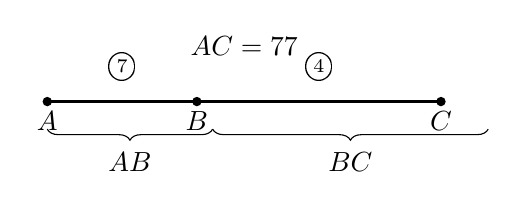
\begin{tikzpicture}[x=1cm,y=1cm,baseline=(current bounding box.center)]
  \draw[line width=1.05pt] (0,0) -- (5.0,0);
  \fill (0,0) circle (1.7pt) node[below] {$A$};
  \fill (1.9,0) circle (1.7pt) node[below] {$B$};
  \fill (5.0,0) circle (1.7pt) node[below] {$C$};
  \draw[decorate,decoration={brace,amplitude=4pt,mirror}] (0,-0.35) -- (2.1,-0.35) node[midway,below=5pt] {$AB$};
  \draw[decorate,decoration={brace,amplitude=4pt,mirror}] (2.1,-0.35) -- (5.6,-0.35) node[midway,below=5pt] {$BC$};
  \node[above=4pt] at (0.95,0) {\textcircled{\scriptsize 7}};
  \node[above=4pt] at (3.45,0) {\textcircled{\scriptsize 4}};
  \node[above=13pt] at (2.5,0) {$AC=77$};
\end{tikzpicture}
  \end{diagramcoltikz}
  \par\medskip
\end{problem}


\needspace{8\baselineskip}

\begin{problem}[points=6]
  \noindent
  \begin{minipage}[t]{\dimexpr\linewidth-60mm-6mm\relax}
    \vspace{0pt}
    射线 $OB$ 在 $\angle AOC$ 内部。若 $7\angle AOB=4\angle BOC$，且 $\angle AOC=121^\circ$，求 $\angle BOC$。  图上份数：____；比例方程：________________；答案：____。
  \end{minipage}\hfill
  \begin{diagramcoltikz}{60mm}{在图上标：左角 4 份，右角 7 份。}
  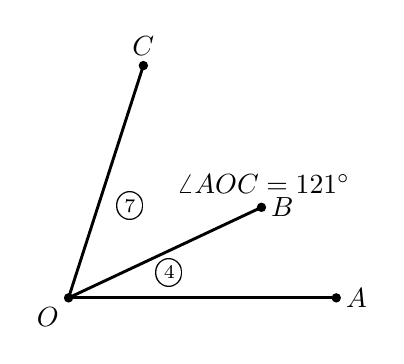
\begin{tikzpicture}[x=1cm,y=1cm,baseline=(current bounding box.center)]
  \coordinate (O) at (0,0);
  \coordinate (A) at (3.4,0);
  \coordinate (B) at (2.45,1.15);
  \coordinate (C) at (0.95,2.95);
  \draw[line width=1.05pt] (O) -- (A);
  \draw[line width=1.05pt] (O) -- (B);
  \draw[line width=1.05pt] (O) -- (C);
  \fill (O) circle (1.7pt) node[below left] {$O$};
  \fill (A) circle (1.7pt) node[right] {$A$};
  \fill (B) circle (1.7pt) node[right] {$B$};
  \fill (C) circle (1.7pt) node[above] {$C$};
  \node at (1.28,0.28) {\textcircled{\scriptsize 4}};
  \node at (0.78,1.12) {\textcircled{\scriptsize 7}};
  \node[right] at (1.25,1.45) {$\angle AOC=121^\circ$};
\end{tikzpicture}
  \end{diagramcoltikz}
  \par\medskip
\end{problem}



\end{document}
